\documentclass[journal,12pt,twocolumn]{IEEEtran}

\usepackage{graphicx}
\usepackage{setspace}
\usepackage{gensymb}
\singlespacing
\usepackage[cmex10]{amsmath}
\usepackage{amssymb}
\usepackage{xurl}
\usepackage{tabularx}
\usepackage{amsthm}
\usepackage{comment}
\usepackage{mathrsfs}
\usepackage{txfonts}
\usepackage{stfloats}
\usepackage{bm}
\usepackage{cite}
\usepackage{cases}
\usepackage{subfig}
\usepackage{arydshln}
\usepackage{longtable}
\usepackage{multirow}

\usepackage{enumitem}
\usepackage{mathtools}
\usepackage{steinmetz}
\usepackage{tikz}
\usepackage{circuitikz}
\usepackage{verbatim}
\usepackage{tfrupee}
\usepackage[breaklinks=true]{hyperref}
\usepackage{graphicx}
\usepackage{tkz-euclide}
\usetikzlibrary{automata, positioning}
\usetikzlibrary{calc,math}
\usepackage{listings}
    \usepackage{color}                                            %%
    \usepackage{array}                                            %%
    \usepackage{longtable}                                        %%
    \usepackage{calc}                                             %%
    \usepackage{multirow}                                         %%
    \usepackage{hhline}                                           %%
    \usepackage{ifthen}                                           %%
    \usepackage{lscape}     
\usepackage{multicol}
\usepackage{chngcntr}
\usepackage{blkarray}

\DeclareMathOperator*{\Res}{Res}

\renewcommand\thesection{\arabic{section}}
\renewcommand\thesubsection{\thesection.\arabic{subsection}}
\renewcommand\thesubsubsection{\thesubsection.\arabic{subsubsection}}

\renewcommand\thesectiondis{\arabic{section}}
\renewcommand\thesubsectiondis{\thesectiondis.\arabic{subsection}}
\renewcommand\thesubsubsectiondis{\thesubsectiondis.\arabic{subsubsection}}


\hyphenation{op-tical net-works semi-conduc-tor}
\def\inputGnumericTable{}                                 %%

\lstset{
%language=C,
frame=single, 
breaklines=true,
columns=fullflexible
}
\begin{document}


\newtheorem{theorem}{Theorem}[section]
\newtheorem{problem}{Problem}
\newtheorem{proposition}{Proposition}[section]
\newtheorem{lemma}{Lemma}[section]
\newtheorem{corollary}[theorem]{Corollary}
\newtheorem{example}{Example}[section]
\newtheorem{definition}[problem]{Definition}

\newcommand{\BEQA}{\begin{eqnarray}}
\newcommand{\EEQA}{\end{eqnarray}}
\newcommand{\define}{\stackrel{\triangle}{=}}
\bibliographystyle{IEEEtran}
\raggedbottom
\setlength{\parindent}{0pt}
\providecommand{\mbf}{\mathbf}
\providecommand{\pr}[1]{\ensuremath{\Pr\left(#1\right)}}
\providecommand{\qfunc}[1]{\ensuremath{Q\left(#1\right)}}
\providecommand{\sbrak}[1]{\ensuremath{{}\left[#1\right]}}
\providecommand{\lsbrak}[1]{\ensuremath{{}\left[#1\right.}}
\providecommand{\rsbrak}[1]{\ensuremath{{}\left.#1\right]}}
\providecommand{\brak}[1]{\ensuremath{\left(#1\right)}}
\providecommand{\lbrak}[1]{\ensuremath{\left(#1\right.}}
\providecommand{\rbrak}[1]{\ensuremath{\left.#1\right)}}
\providecommand{\cbrak}[1]{\ensuremath{\left\{#1\right\}}}
\providecommand{\lcbrak}[1]{\ensuremath{\left\{#1\right.}}
\providecommand{\rcbrak}[1]{\ensuremath{\left.#1\right\}}}
\theoremstyle{remark}
\newtheorem{rem}{Remark}
\newcommand{\sgn}{\mathop{\mathrm{sgn}}}
\providecommand{\abs}[1]{\vert#1\vert}
\providecommand{\res}[1]{\Res\displaylimits_{#1}} 
\providecommand{\norm}[1]{\lVert#1\rVert}
%\providecommand{\norm}[1]{\lVert#1\rVert}
\providecommand{\mtx}[1]{\mathbf{#1}}
\providecommand{\mean}[1]{E[ #1 ]}
\providecommand{\fourier}{\overset{\mathcal{F}}{ \rightleftharpoons}}
%\providecommand{\hilbert}{\overset{\mathcal{H}}{ \rightleftharpoons}}
\providecommand{\system}{\overset{\mathcal{H}}{ \longleftrightarrow}}
	%\newcommand{\solution}[2]{\textbf{Solution:}{#1}}
\newcommand{\solution}{\noindent \textbf{Solution: }}
\newcommand{\cosec}{\,\text{cosec}\,}
\providecommand{\dec}[2]{\ensuremath{\overset{#1}{\underset{#2}{\gtrless}}}}
\newcommand{\myvec}[1]{\ensuremath{\begin{pmatrix}#1\end{pmatrix}}}
\newcommand{\mydet}[1]{\ensuremath{\begin{vmatrix}#1\end{vmatrix}}}
\newcommand*{\permcomb}[4][0mu]{{{}^{#3}\mkern#1#2_{#4}}}
\newcommand*{\perm}[1][-3mu]{\permcomb[#1]{P}}
\newcommand*{\comb}[1][-1mu]{\permcomb[#1]{C}}
\numberwithin{equation}{subsection}
\makeatletter
\@addtoreset{figure}{problem}
\makeatother
\let\StandardTheFigure\thefigure
\let\vec\mathbf
\renewcommand{\thefigure}{\theproblem}
\def\putbox#1#2#3{\makebox[0in][l]{\makebox[#1][l]{}\raisebox{\baselineskip}[0in][0in]{\raisebox{#2}[0in][0in]{#3}}}}
     \def\rightbox#1{\makebox[0in][r]{#1}}
     \def\centbox#1{\makebox[0in]{#1}}
     \def\topbox#1{\raisebox{-\baselineskip}[0in][0in]{#1}}
     \def\midbox#1{\raisebox{-0.5\baselineskip}[0in][0in]{#1}}
\vspace{3cm}
\title{ ASSIGNMENT 3}
\author{HARITHA R\\ AI20BTECH11010}
\maketitle
\newpage
\bigskip
\renewcommand{\thefigure}{\arabic{figure}}
\renewcommand{\thetable}{\arabic{table}}
Download all python codes from
\begin{lstlisting}
https://github.com/harithar1234/EE3900-Haritha/blob/main/assignment3/assignment3.py
\end{lstlisting}
\section*{QUESTION}
\textbf{Construction/Q 2.18}
\begin{enumerate}
Draw a circle with centre $B$ and radius 6.  If $C$ be  a point 10 units  away from its 
centre, construct the pair of tangents $AC$ and $CD$ to the 
circle.
\end{enumerate}
\section*{SOLUTION}
\begin{enumerate}
Let the center of the circle be 
\begin{align}
    \vec{B} = \myvec{0 \\ 0}
\end{align}
and radius = 6 units.\\
Therefore the equation of the circle is given by
\begin{align}
    \vec{x} = \myvec{0 \\ 0} + 6\myvec{\cos \theta \\ \sin\theta}
\end{align}
The tangent are drawn from a point $\vec{C} \myvec{10 \\ 0}$ on the x-axis which intersect the circle at point $\vec{A}$ and $\vec{D}$.\\
Since, point $\vec{A}$ lie on the circle ,
\begin{align}
    &&\norm{\vec{AB}} =6\\
    &\implies& \norm{\vec{A-B}}=6\\
    &\implies& \norm{\vec{A}}=6
\end{align}
In any circle tangent is perpendicular to the radius.
So in $\triangle ABC$, $\vec{BA}$ and $\vec{CA}$ are perpendicular
\begin{align}
    &&\vec{(BA)}^\top \vec{(AC)} &= 0\\
    &\implies& \vec{(B-A)}^\top \vec{(A-C)} &= 0\\
    &\implies& \vec{B^\top A} - \vec{B^\top C} - \norm{\vec{A}}^2 + \vec{A^\top C} &= 0
\end{align}
since $\vec{B^\top A}=0$ and $\vec{B^\top C}=0$
\begin{align}
    && - \norm{\vec{A}}^2 + \vec{C^\top A} &= 0\\
    &\implies& \vec{C^\top A} &= \norm{\vec{A}}^2\\
    &\implies& \vec{C^\top A} &= 36 \label{1}
\end{align}
Now, \eqref{1} can be rewritten as
\begin{align}
&&\myvec{10 & 0}\vec{A} &= 36\\
&\implies& \myvec{1 & 0}\vec{A} &= 3.6\\
&\implies& \vec{A} &= \myvec{3.6 \\ 0} + \lambda \myvec{0 \\ 1}\\
&\implies& \vec{A} &= \vec{q} + \lambda \vec{m}
\end{align}
where, $\vec{q} = \myvec{3.6 \\ 0}$ and $\vec{m} = \myvec{0 \\ 1}$\\
Now, we know that
\begin{align}
&&\vec{\norm{A}^2} &= 36\\
&\implies& \norm{\vec{q}+\lambda \vec{m}}^2 &= 36\\
&\implies& (\vec{q}+\lambda \vec{m})^\top(\vec{q}+\lambda \vec{m})&= 36\\
&\implies& \norm{\vec{q}}^2 + 2\vec{q}^\top \lambda \vec{m} + \lambda^2 \norm{\vec{m}}^2 &= 36
\end{align}
Since, $\vec{q}^\top \vec{m} = 0$ $\implies$
$2\vec{q}^\top \lambda \vec{m} = 0$
\begin{align}
&\implies&\lambda^2 &= \cfrac{36-\norm{\vec{q}}^2}{\norm{\vec{m}}^2}\\
&\implies& \lambda^2 &= \cfrac{36-(3.6)^2}{1}\\
&\implies& \lambda &= \pm 4.8
\end{align}\\
Therefore, $\vec{A} = \myvec{3.6 \\ 4.8}$ and $\vec{D} = \myvec{3.6 \\ -4.8}$ 
\begin{center}
    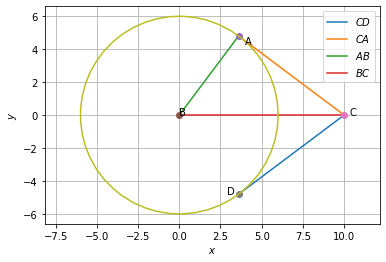
\includegraphics{assignment3.png}
\end{center}
\end{enumerate}

\end{document}